\startchapter{AI-driven Software Engineering}
\label{chapter:Exp}

The current approaches focus on programming-in-the-small i.e, on individual lines of code. 
Code language models have focused (effectively!) on source code as language, implying the task is to predict the next token or series of tokens.
Thus support is for software \textit{coding} rather than software \emph{engineering}. 
What might AI support for software engineering require? 

There are areas of code suggestions that are not easily fixable or at least, not detectable efficiently before training or recommendation is required, at the time-scale of code completion (less than one second) \cite{}.
These problems align with a software abstraction hierarchy that sees code compilation and syntax checking at the least abstract level, and software architecture analysis and design at the most abstract level.
Figure \ref{fig:levels} exemplifies this. \neil{adapt for this paper - add AI, add line of tradeoff}
As we descend the levels, we have software concepts that are more difficult to automate (design rules vs code smells), that are nonetheless more important for software quality attributes (QA). 
We suggest that similarly, AI will struggle to offer useful suggestions lower down the list. 
The question remains where we stand today, and where the line (or area) exists between places where the AI should drive, and where a human engineer should take control.

\begin{figure}
    \centering
    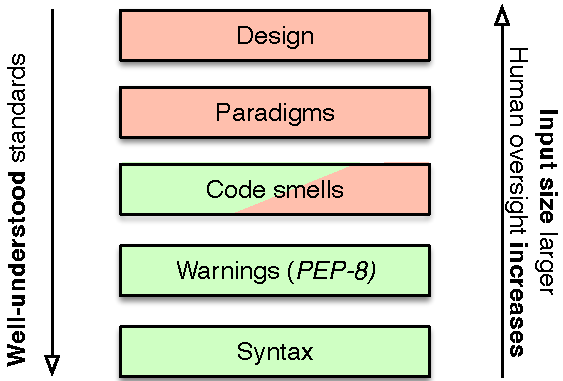
\includegraphics[width=.5\linewidth]{Figures/taxonomy-copilot.pdf}
    \caption{Hierarchy of software abstractions. Syntax reflects syntactically correct code and is warned by the compiler. Warnings include `-w' style compiler flags. Smells are aspects of source code that are sub-optimal by general acceptance; paradigms are idioms and good practices for languages and problems areas such as mobile computing. Finally, design refers to optimal design approaches for system qualities.}
    \label{fig:levels}
\end{figure}

We consider three scenarios. 
One is the way Copilot and AI-driven development manage language idioms.
A second is the way best practices are dealt with.
% \neil{third? maybe SQ smells design smells.}.

\subsection{Paradigms and Idioms}
Paradigms and idioms are our taxonomy's third level of software abstraction. 
This level requires the code suggested by \cct{} to satisfy all the previous levels of abstractions and use common paradigms and language idioms in its code suggestions. 
These include common practices of solving a programming task. 

Returning to our running example of performing a sorting operation on a list of numbers. 
To satisfy this level of abstraction, \cct{} should suggest a syntactically correct list sorting code, using idiomatic ways in its code suggestions, like the Pythonic way of swapping items in a list~(line 5 in figure~\ref{fig:idioms}), As opposed to suggesting non-idiomatic approaches like creating another temporary variable to swap items in a list shown in correctness level~(figure~\ref{fig:correctness}).

Figure~\ref{fig:idioms} shows the sorting example and the Python code suggestions from \cct{} at this abstraction level.

\begin{figure}[hbt!]
    \centering
\begin{tcolorbox}[title=Idioms level suggestion for sort routine,boxsep=.15mm]
    %https://tex.stackexchange.com/questions/337909/tcolorbox-tcbline-style
\textbf{Human Input:}
\begin{lstlisting}[language={Python}]
# sorting a list
arr = [2,4,1,3,7,5]
\end{lstlisting}
\tcbline
\textbf{\cct{} suggestion:}
\begin{lstlisting}[language={Python}]
n = len(arr)
for i in range(n):
	for j in range(n-1):
		if arr[j] > arr[j+1]:
			arr[j], arr[j+1] = arr[j+1], arr[j]
print(arr)
\end{lstlisting}
\end{tcolorbox}
    \caption{Code suggestion of \cct{} at paradigms and idioms level.}
    \label{fig:idioms}
\end{figure}

The goal of this software abstraction level in the taxonomy is for \cct{} to detect and use commonly known idiomatic approaches and paradigms that occur in public code in its suggestions for suggesting code to solve a programming task.

The capabilities required by \cct{} to satisfy paradigms and idioms level of software abstraction are as follows:
\begin{enumerate}
    \item Identify common patterns like paradigms and language idioms in public code repositories~(training data).
    \item Use paradigms and language idioms in suggesting solutions for a programming task.
    \item Satisfy requirements of all the levels below paradigms and idioms in our taxonomy.
\end{enumerate}


\section{Code Review Best Practices}
We considered best practices for code review in JavaScript development. 
This aligns with the Code Smell level (middle tier) in our taxonomy. 
To ground our practices we relied on the AirBNB JavaScript coding style guide~\cite{airbnb_code}, a widely used coding style and code review standard. 
The AirBNB standard contains a variety of best practices. 
To scope our approach, we chose practices that were closer to the the design level of our taxonomy, rather than the code level (e.g., trailing comma use in Javascript).

% For example, in JavaScript, callback api was used in the past to achieve concurrency which were replaced by promises. We checked if copilot suggests code which is specifically mentioned in the JavaScript documentation as a bad practice or an anti-pattern. Bad Practices in using promises for asynchronous JavaScript like not returning promises after creation, forgetting to terminate chains without catch statement, which are explained in documentation\footnote{\url{https://developer.mozilla.org/en-US/docs/Web/JavaScript/Guide/Using_promises}} and StackOverflow\footnote{\url{https://stackoverflow.com/questions/30362733/handling-errors-in-promise-all/}} are not known to copilot and suggested code with those common anti-patterns as they occur more frequently in copilot training data.

\noindent\textbf{Method:} We chose 5 JavaScript coding standards from the AirBNB JavaScript coding style guide~\cite{airbnb_code}. We considered it a match if Copilot suggested the recommended way in the first 2 suggestions, but note if the recommended way appeared any of the top 10 suggestions. 
Below is the list of five best practices we tested:
% \neil{i think a quick list listing the chosen standards would help, alongside the place the suggestion occurred (e.g.).}

\begin{itemize}
    \item Practice 1: Object Shorthand: Usage of object method shorthand (no suggestion matched)
    \item Practice 2: Array Creating Constructor (place: 6th)
    \item Practice 3: Copying Array Contents (no suggestion matched)
    \item Practice 4: Logging a Function (no suggestion matched)
    \item Practice 5: Exporting a Function (no suggestion matched)
\end{itemize}

Copilot failed to suggest the recommended way for all five standards we tested, i.e, Copilot did not have the recommended way in its top two suggestions. Only 1 out of 5 standards had the recommended way in the top 10 suggestions. 

Below is an example of logging a function (Practice 4). 
We first show the user input that triggers Copilot, the top suggestion by Copilot (i.e. model output) and the recommended way suggested by the AirBNB coding style guide~\cite{airbnb_code}.

\begin{tcolorbox}[title=Logging a Function,boxsep=.5mm]
    %https://tex.stackexchange.com/questions/337909/tcolorbox-tcbline-style
\textbf{Human Input:}
\begin{lstlisting}[language=JavaScript]
// logging function

class foo {
    bar ()
\end{lstlisting}
\tcbline
\textbf{Copilot Suggestion:}
\begin{lstlisting}[language=JavaScript]
{
    console.log('bar');
    }
}
\end{lstlisting}
\tcbline
\textbf{Ideal way\footnote{source~\cite{airbnb_code}}:}
\begin{lstlisting}[language=JavaScript]
class foo {
    bar (){ 
    console.log(this.bar) ;
}}
\end{lstlisting}
\end{tcolorbox}

\section{Design Smells}
Currently, Copilot does not support multi-file input, So it is not possible to evaluate its design suggestions, as software development process may include multiple folders with a file structure. 
Making Code completion tools adapt their suggestions to context specific issues such as variable naming conventions and formatting would be challenging as the existing guidelines are not standard in this space and mostly depend on context, The training dataset for AI driven development should also include rules such as idioms, best practices before tackling design level problems.
% Design smells or arch smells (Tushar Sharma)
\section{Limitations}
Access to Copilot

Copilot is very sensitive to input. This hurts replicability as a different formulation of the problem might well produce a totally different set of suggestions. 
Thus a reasonable concern is that our (human) input is unfair to Copilot, and with some longer suggestions, the tool would generate the correct idiom. \neil{can we try this? }\rohith{idioms are mostly one lined, and longer inputs/suggestions could be described as bad practices/design smells}
Our intention is admittedly to show where Copilot is not able to consistently generate the preferred answer. We biased our evaluation to highlight this by choosing input that simulates what a less experienced programmer might choose. But this is reasonable: for one, these are precisely the developers likely to use Copilot suggestions, and unlikely to know the idiomatic usage; more importantly, a lack of suggestion stability seems to come with its own set of challenges (to use an analogy, we would expect every Tesla to make the same choice when confronted with the same circumstances). %this gets to the top levels of Koopmann's pyramid.

Working with GitHub's API - not open

OpenAI and open source

Ethics about suggestions - different when suggestions are much broader e.g. what sort algorithm to use. Not just a technical question and much more challenging ethically than flash fill. 
